\section{Test Plan}
This chapter will introduce the overall test plan for this project, and it is based on the IEEE 829 Standard for Software Test Documentation[link to reference]. Some parts of the standard was not deemed to be appropriate for this project and not included as a result. The purpose of this document is to structure the way tests are performed and recorded, assign responsibilities for the testing process as a whole, and to give an outline for the schedule of when the different tests should be performed.

\subsection{Testing Approach}
The testing methods used for this project is discussed in detail in the pre- study. To sum up, we have opted to utilize both black and white box testing in this project. We will write and run unit tests throughout the implementation process together with an automated test framework. The test cases included in the report will be component, system, user and acceptance tests. If additional requirements are added to the system during the Scrum process, new test cases will be created to test the desired functionality.

\subsubsection{Non- Functional Requirements}
The aren’t many non- functional requirements that are essential in this project. It is a proof of concept type of project and the main goal is to prove that the solutions we come up with will get the job done. As a result, tests for common non- functional requirements like performance and security will not be included in the test cases. 

One non- functional requirement worth writing tests for though is usability. The object of the project is to deliver a system that eases the workflow of specific users, and to achieve this we need to develop a system with a large degree of usability. Thats why usability tests will be included in the test cases, in the form of user testing(interviews).

\subsubsection{Testing Process Timeline}
Figure~\ref{figure:testOutline} outlines when the different tests will be performed during the Scrum process. Unit testing will be done throughout the development process in every sprint. Every part of the code implemented should have its own unit tests. Component testing will be done as separate components are finished, typically towards the end of the sprints. Acceptance testing with the customer will be performed in the sprint demo at the end of each sprint. At these demos it will be tested whether the agreed upon functionality for that sprint is actually implemented. System testing will be performed when we have an entire system to test, i.e. when we have implemented some parts of each component needed for the entire system to work. This will likely not be the case until the end of the second sprint. User testing will also be performed in the later sprints, when we have a complete system to present to the test users. Release testing will be performed at the end of the last sprint, to see if the agreed upon functionality for the entire project is indeed present in the system.

\begin{figure}
\centering
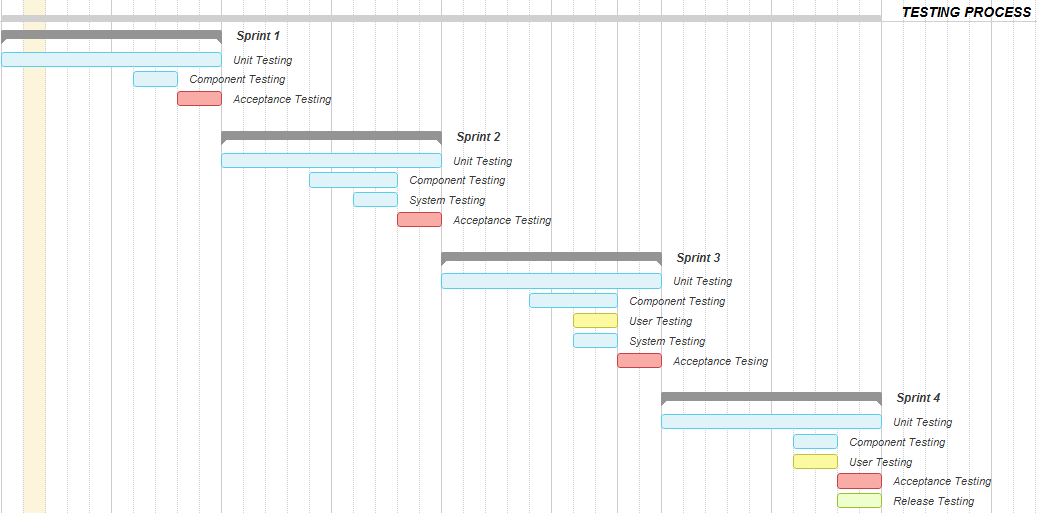
\includegraphics[width=6in]{image/testingProcess.png}
\caption{Testing Process Timeline}
\label{figure:testOutline}
\end{figure}

\subsection{Templates}
The templates stated in Table~\ref{table:testcase} and Table~\ref{table:testreport} will be used to create test cases and to record the results of them.

\begin{table}
\caption{Test Case Template}
\centering
\begin{tabular}{ l l }
\hline
 Item            & Description                                                              \\ 
\hline
 Description     & Description of requirement                                               \\ 
 Tester          & The person responsible for performing the specific test                  \\ 
 Preconditions   & The condition that has to be fulfilled before the execution of this test \\ 
 Feature         & The feature of the system that is to be tested                           \\ 
 Execution steps & Steps to be executed in this test case                                   \\ 
 Expected result & The expected result of the test                                          \\
\hline
\end{tabular}
\label{table:testcase}
\end{table}

\begin{table}
\caption{Test Report Template}
\centering
\begin{tabular}{ l l }
\hline
Item        & Description                             \\ 
\hline
Test ID     & The ID of the given test                \\ 
Description & Description of the requirement          \\ 
Tester      & The person executing the test           \\ 
Date        & The date the test was performed         \\ 
Result      & The result of the test, success or fail. Comment will be added if deemed needed \\
\hline
\end{tabular}
\label{table:testreport}
\end{table}

\subsection{Responsibilities}
The test manager is the one with overall responsibility of the quality of the test plan, and that it will be executed according to the schedule. The person writing test cases and recording test results is responsible for adhering to the templates included in this document.

Each person is responsible for creating unit tests for their own code, and to run these with the automated test framework during development. This will be done to perform continuous testing of the system, and uncover if any new code break some of the previous tests.

We will mainly use someone different to perform the actual test cases than the person who wrote the specific code segment. This is done to achieve as little ownership of the code as possible on part of the tester. But as we are short on manpower and time we can’t guarantee that this is always the case. 

The test cases will be performed towards the end of each sprint when the relevant functionality is implemented. The test will be performed at a time which allows the developers to fix any uncovered bugs in the system before the sprint is ended. 

\subsection{Test Criteria}
A test is considered passed when it achieves the expected result. A test will be considered to have failed if the result of the test differs from the expected one. If we feel a pass/fail of a specific test needs an explanation this will be noted as a comment in the result.